\chapter{Metodologia}\label{meto}

O processo para construir o modelo preditivo foi o CRISP -- DM. forneça informação suficiente a um gestor para decidir quando e por onde 
enviar uma frota de caminhões por determinada rodovia que apresente retenções crescentes de logística de cargas. As soluções disponíveis que 
existem tais como; Google Maps, Waze e outros dessa natureza somente exibem informações momentâneas, produzidas e compartilhadas pelos utilizadores 
dos aplicativos ou por informações provindas de GPS, contudo não analisam dados históricos dessas rodovias nem fazem predições futuras sobre o 
comportamento delas. \\

\section{Plano geral da metodologia}

A metodologia da pesquisa contempla um plano em três etapas, cada uma dividida em fases atinentes.
As duas primeiras etapas da nossa metodologia completam o ciclo do processo CRISP-DM.
A terceira etapa é o ``front-end'', onde são plotados no mapa os pontos críticos da rotas.

\pagebreak

A figura a seguir ilustra essa metodologia descrita graficamente, onde as três etapas são representadas por retângulos.
 
\begin{figure}[ht]
\centering
\caption{Etapas da gerais da metodologia}
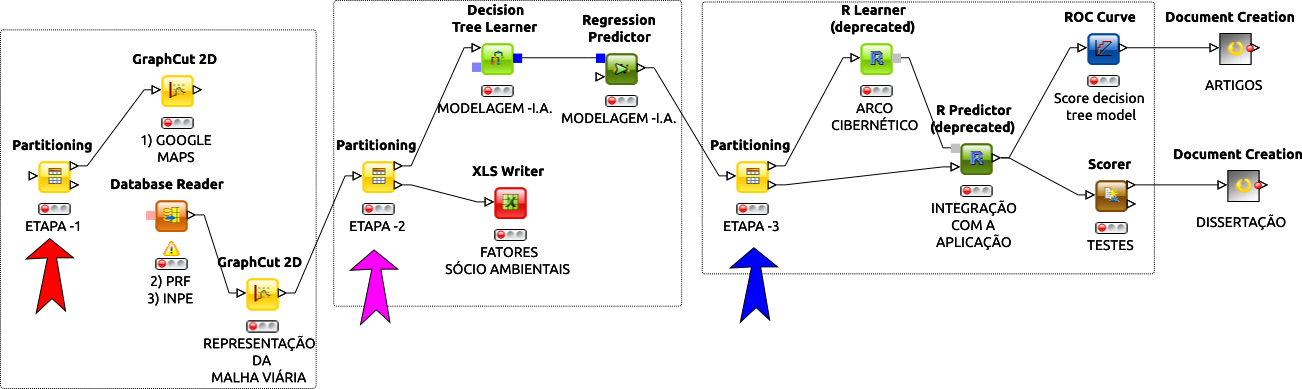
\includegraphics[width=160mm, height=70mm]{Figuras/BigData/Etapas.png}
\end{figure}

A \textbf{etapa 1} contempla a fases da coleta das bases de dados históricas, preparação dos dados e construção das variáveis do modelo preditivo.
\begin{enumerate}
 \item O modelo preditivo integra várias bases de dados, tais como: Polícia Rodoviária Federal -- PRF, Batalhão de Polícia de Transito -- BPRv e dados históricos 
       do Instituto de Pesquisas Espaciais -- INPE ou dos dados de precipitações pluviométricas do ``European Centre for Medium-Range Weather -- ECMWF.
 
 \item Algumas dessas informações também estão disponíveis em base de dados abertas, como sugere o Portal da Transparência, nos servidores da PRF além de outras informações para complementar o sistema estão 
       disponíveis na Internet sendo atualizadas pela PRF através de uma API aberta, esta pode ser configurável para se ligar ao nosso sistema.
\end{enumerate}

 
O segunda \textbf{etapa 2} consiste na Mineração dos dados, tendo como ''inputs`` a etapa anterior; aplicar as técnicas de IA nas variáveis do sistema preditivo.
%Propomos inicialmente a Regressão Logística e Árvores de decisão, testes iniciais e depuração do modelo. transformar os dados provenientes do modelo preditivo em coordenadas geográficas, isto é:
Os ''outputs`` dessa etapa consiste em transformar os dados provenientes mineração em coordenadas geográficas, isto é: em latitude e longitude.  
 
A \textbf{terceira} e última etapa da metodologia contempla:
 \begin{enumerate}
  \item A malha viária representada em mapas de bases vetoriais;
  \item Um ambiente de simulação interativa que utiliza uma plataforma baseada na API do Google Maps.
  \item Um módulo dinâmico onde são capturados ``feeds'' de redes sociais, por exemplo pelo Twitter. 
	Essa técnica faz um arco cibernético mantendo o sistema atualizado.
\end{enumerate}

As coordenadas geográficas, ``outputs'' da etapa 2, são agrupadas a priori formando ''cluster`` de dados 
a serem exibidos nos mapas vetoriais das APIs correspondentes.

A representação da malha viária, que acopla a estrutura dinâmica com a estrutura estática, é o ``front-end'' da metodologia. 
Esta etapa permite uma contraposição ao modelo preditivo na perspectiva do usuário gestor. 
Isso pois, modelos preditivos com o passar do tempo tendem a desfasar-se, contudo este módulo permite visualização
instantânea do ambiente das rodovias. 
 


\section{Modelo preditivo}

O modelo preditivo foi construído utilizando bases de dados históricas da PRF (de acidentes e de paralisações ex: protestos) entre Janeiro de 2007 a 
Dezembro 2015. As bases de dados do Batalhão de Polícia de Rodoviária estadual -- BPRv vieram entre Janeiro/2010 a Julho/2016, cortes em ambas as bases foram 
feitos para adequar as datas. Essas bases de dados são integradas gerando um único e complexo modelo preditivo que será acoplado a estrutura dinâmica.


%\pagebreak

\section{Reflexão sobre as tecnologias utilizadas no modelo preditivo}\label{result}

Não existe uma técnica de mineração que generalize os mais diversos ambientes preditivos, mas sim um ``pool'' dessas técnicas onde uma complementa outra.

As técnicas preditivas tradicionais que contemplam análise de grandes massas de dados como base homogêneas.

são possíveis quando adaptadas para uma forma comparável à que
foram inicialmente concebidas, por que as variáveis em uma base de dados a priori guardam pouca relação as variáveis de outra base de dados.
neste caso essas variáveis ou são excluídas ou são transformadas a fim de ``guardarem'' um correlação com a outra base de dados. 

Na fase de transformação de dados, onde são criadas novas variáveis, a proximidade entre as
bases heterogêneas deverão se estreitam. 
Nesta pesquisa, bases heterogêneas foram integralizadas num única grande base, onde as variáveis independentes foram
em sua maioria preservadas e/ou construídas novas, nas bases onde não haviam correspondência, respeitando a lógica do negócio.\\
A tabela a seguir descreve as variáveis originais na base de dados de acidentes da PRF 


\section{Extração do conhecimento}

As técnicas como Redes Neurais Artificias (MLP) \cite{DecisaoCredito}, Árvores de decisão (CART) \cite{DataMining}, Regressão logística (MLR) 
\cite{RegrecaoLog} fornecem visão generalizada dos fatores preponderantes, levantando padrões ocultos nos dados. Esta fase é conhecida como 
Aprendizagem de Máquina (acrônimo de Machine Learning)

\begin{itemize}
 \item[a] Redes Neurais Artificias do tipo \textit{ Multi Layer Perceptron}  -- (MLP) têm capacidade de receber várias entradas ao mesmo tempo e distribuí-las de maneira organizada, além 
	  são simples de implementar e trazem resultados satisfatórios em grandes bases de dados.
 
 \item[b] Árvores de decisão para classificar acidentes do tipo \textit{ Classification and Regression Tree}  -- (CART) foi empregue por Pakgohar et al no artigo 
	  \textit{The role of human factor in incident and severity of road crashes based on the CART and LR regression a data mining approach}  com nível de acurácia próximo aos 80\%

 \item[c] Regressão logística tipo \textit{Multinomial Logistic Regression} -- (MLR) fornece a possibilidade de aprofundamento em vários níveis de busca sendo a mais apropriada, já que Regressão logística 
	  tradicional não permite aprofundamento desse tipo no espaço de busca.
\end{itemize}


\pagebreak

\section{Acoplamento com a estrutura dinâmica}

A estrutura dinâmica é composta por duas API's, uma disponibilizada pela Google, através do Google Maps que está atualmente na versão V3 e 
outra uma API do Twitter. A API do Google Maps proporciona uma ``leitura'' atualizada em forma de mapa no momento em que a estrutura dinâmica ``roda''. 

A API do Twitter também tem a possibilidade de atualizar o modelo preditivo, contudo o objetivo desta é faz um Arco cibernético, 
retroalimentando todo o sistema com novas informações, pensamos que isso permite um visualização instantânea do ambiente como um todo.

Os ``feeds'' das redes sociais como o Twitter permitem analisar o contexto das rodovias com defasagem temporal 
pequena, os utilizadores dessas redes sociais inclusive a PRF atualizam as redes sociais com dados sempre que há uma ocorrência por essas 
A monitoração dessas redes sociais se faz por Mineração em textos, são verificas palavras chaves como: protestos, acidentes e outras.



\begin{figure}[ht]
\centering
\caption{Etapas da metodologia}
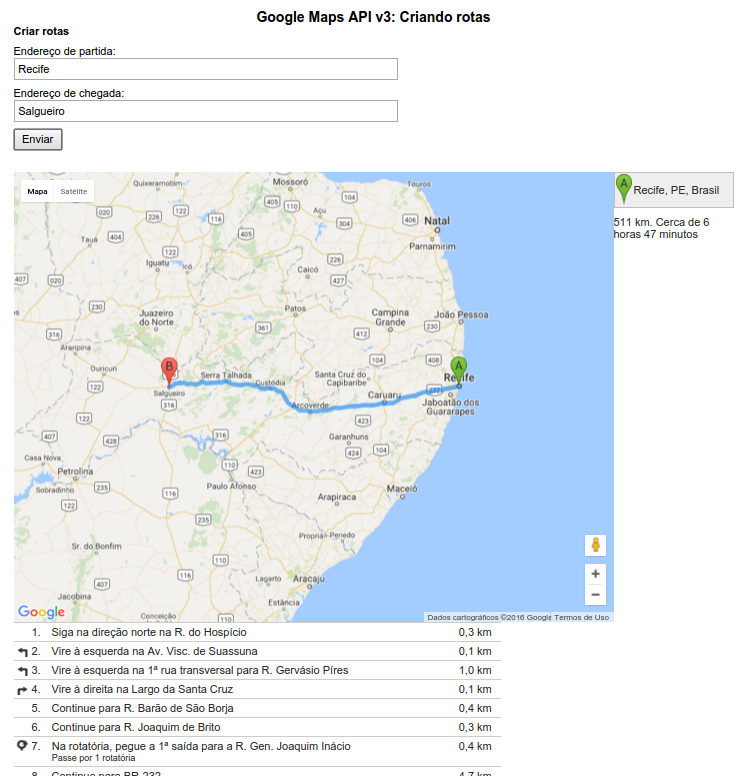
\includegraphics[width=150mm, height=130mm]{Figuras/Cronograma/GoogleMaps.png}
\end{figure}